\chapter{Instanciación  y uso del framework}
En esta sección se explica como instanciar el framework para su uso, brindando algunos ejemplos concretos.

Una vez instalado el framework el siguiente paso es instanciarlo para usarlo. La instanciación puede ser manual o usando el generador de clases de Gradle.


\section{Instanciación manual} \label{sec:instanciacion_manual}
Una vez agregada la librería de Samplers al proyecto, se debe crear un objeto Workflow, agregarle los objetos Steps, y llamar a la activity TakeSampleActivity pasándole el objeto Workflow como parámetro.
También es necesario establecer la configuración general en el método onCreate de la activity principal (main activity) para indicar a donde se enviarán las muestras tomadas con la app.
Se puede usar una activity principal propia o se puede heredar de SamplersMainActivity. En ambos casos se debe hacer lo siguiente:
\begin{itemize}
	\item Establecer la configuración general en el método onCreate de la activity principal:
	
		
\begin{figure}[H]
  \centering
    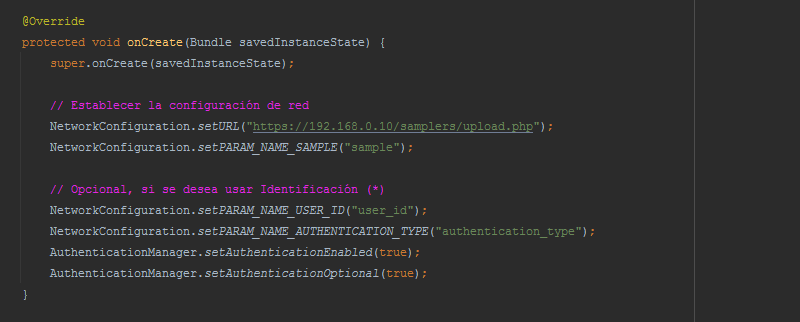
\includegraphics[scale=0.6]{50-anexos/B-uso/configuracion_general.png} 
   \caption{Ejemplo de configuración general}
\end{figure}		
		
		
(*) Ver la sección \ref{sec:usando_autenticacion} para más detalles sobre como usar identificación.


	\item Crear un Workflow. Si se está heredando de SamplersMainActivity se debe hacer sobreescribiendo el método getWorkflow.
	
\begin{figure}[H]
  \centering
    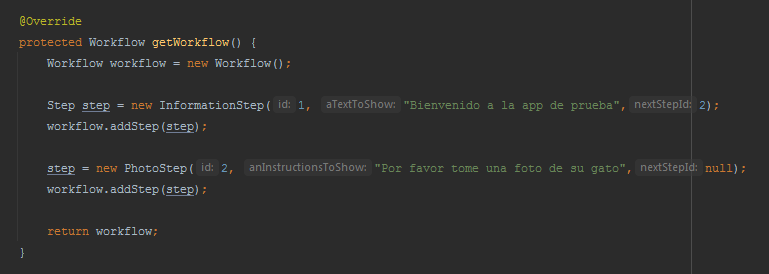
\includegraphics[scale=0.6]{50-anexos/B-uso/get_workflow.png} 
   \caption{Ejemplo de un Workflow que tiene dos Steps. El primero muestra un mensaje de bienvenida y el segundo pide para tomar una foto.}
\end{figure}		
	

Nota: Para ver los distintos Steps que se pueden usar vea la sección \ref{sec:steps_detallados}.

	\item Iniciar la activity TakeSampleActivity. Si se está heredando de SamplersMainActivity esto se hace automáticamente en el método onClick del botón "tomar muestra". De lo contrario, deberá iniciarla de la siguiente forma, en el método onClick de un botón por ejemplo:

\begin{figure}[H]
  \centering
    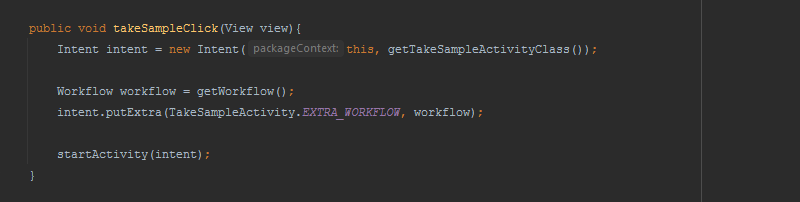
\includegraphics[scale=0.6]{50-anexos/B-uso/take_sample_click.png} 
   \caption{Ejemplo de como iniciar la activity TakeSampleActivity.}
\end{figure}		

\end{itemize}


\section{Instanciación usando el  generador de clases de Gradle}

Básicamente, el generador de clases de Gradle se encarga de hacer una instanciación manual a partir de un archivo de configuración (JSON). Está pensado para desarrolladores que no tienen muchos conocimientos en Android, o para servir de interfaz entre una aplicación que genere apps a través de Samplers.

Los pasos para usar el generador de clases de Gradle son:
\begin{enumerate}
	\item Crear un archivo JSON con el nombre SamplersConfig.json
		\begin{itemize}
			\item El formato y las opciones están explicadas sección \ref{sec:archivo_config_detallado}.
			\item Para validar sintaxis se puede usar por ejemplo el validador online https://jsonformatter.curiousconcept.com que es gratuito.
			\item Al final de esta sección se provee un archivo de ejemplo.
		\end{itemize}
		
	\item Copiar el archivo creado en el item anterior al directorio raíz del proyecto Android creado.
	
	\item Descargar la última versión de los archivos \textbf{samplers.gradle} y \textbf{samplersclassgenerator.jar} del repositorio de Samplers\footnote{https://github.com/cientopolis/samplers/releases/} y copiarlos también al directorio raíz del proyecto Android.
	
	\item Enlazar el archivo samplers.gradle en el archivo \textbf{build.gradle} de la aplicación:
		\begin{itemize}
			\item Android Studio crea por defecto dos archivos build.gradle, uno a nivel de aplicación y otro a nivel de proyecto. Debe usarse el de aplicación.
			\item Al final del archivo build.gradle de aplicación agregar:
\begin{lstlisting}[language=XML, frame=tlbr]
apply from: '../samplers.gradle'
\end{lstlisting}
			\item Al guardar los cambios, Android Studio sugerirá hacer una sincronización del proyecto, hacerla. Esto generará en la aplicación una activity llamada MyMainSamplersActivity en base a las opciones configuradas en el archivo SamplersConfig.json.
			\item Si se necesita volver a generar esta activity (si se quieren modificar algunas opciones por ejemplo ) se puede eliminar la misma, hacer las modificaciones en el archivo SamplersConfig.json y volver a generar el proyecto (en el menu Build -$>$ Make Project)
		\end{itemize}
		
	\item Eliminar o personalizar el archivo \textbf{style.xml} que está en \textbf{res/values} en la aplicación
	
	\item Ejecutar la aplicación y listo.

\end{enumerate}


\section{Secciones del archivo} \label{sec:archivo_config_detallado}

El archivo SamplersConfig.json es un archivo JSON con 3 objetos: project, application y workflow. A continuación se explican en detalle cada uno de ellos.

\subsection{El objeto project}
		
	El objeto project tiene dos campos
	\begin{itemize}
		\item \textbf{app\_path}: Un String con la ubicación del directorio de los fuentes de la aplicación, relativo al directorio del proyecto. Es donde están los archivos -java de la aplicación y donde se creará el archivo MyMainSamplersActivity.java
		\item \textbf{package\_name}: Un String con el nombre del package usado para las activities de la aplicación. Es el package donde la activity MyMainSamplersActivity será agregada.
	\end{itemize}
	
\begin{figure}[H]
  \centering
    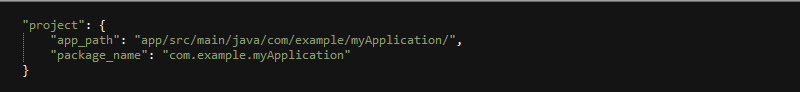
\includegraphics[scale=0.6]{50-anexos/B-uso/json_project.png} 
    \caption{Ejemplo del objeto project.}
\end{figure}	
	
\subsection{El objeto application}
	El objeto application tiene 7 campos, de los cuales 3 son requeridos y los otros 4 opcionales (para habilitar características especiales)
	\begin{itemize}
		\item \textbf{title}: Un String con el nombre de la aplicación.
		
		 \item \textbf{welcomeMessage}: Un String con el mensaje de bienvenida que se mostrará en la activity principal (MyMainSamplersActivity)
		 
		 \item \textbf{networkConfiguration}: Un objeto con la configuración de red que se usará para enviar las muestras al servidor web. Ver mas abajo la configuración de este objeto.
		 
		 \item \textbf{googleMaps\_API\_KEY}: [Opcional] Un String con la API Key de Google. Este campo es necesario si se van a usar los servicios de ubicación y mapas (Location Step y Route Step). La API Key de google se puede obtener desde la página de google developers \footnote{https://developers.google.com/maps/documentation/android-api/signup}.
		 
		 \item \textbf{mainHelpFileName}: [Opcional] Un String con el nombre del archivo HTML que contiene la ayuda principal de la aplicación. Este archivo debe estar junto con el archivo SamplersConfig.json. Ver la sección \ref{sec:mostrar_ayuda} para mas detalles.
		 
		 \item \textbf{authenticationEnabled}: [Opcional] Un boolean que indica si se usará autenticación (true) o no (false). Si se omite este campo se asume false. Ver la sección Usando Autenticación para mas detalles.
		 
		 \item \textbf{authenticationOptional}: [Opcional] Un boolean que indica si la autenticación será opcional (true) o requerida (false). Si se omite este campo se asume true (autenticación opcional). Este campo solo tiene sentido si se usa autenticación. Ver la sección Usando Autenticación para mas detalles.
		 
	\end{itemize}
	
	
	El objeto \textbf{networkConfiguration}:
	El objeto networkConfiguration contiene la configuración de red que se usará para enviar las muestras al servidor web. Tiene 4 campos, de los cuales 2 son requeridos y los otros 2 opcionales.
	
	\begin{itemize}
	
		\item \textbf{url}: Un String con la URL del servidor web al cual se le enviaran las muestra con un mensaje HTTP POST.
		
		\item \textbf{paramName}: Un String con el nombre del parámetro dentro del mensaje HTTP POST en el que se enviará la muestra.
	
		\item \textbf{paramNameUserId}: [Opcional] Un String con el nombre del parámetro dentro del mensaje HTTP POST en el que se enviará el id del usuario que envía la muestra. Este campo solo es necesario si se usa autenticación. Ver la sección Usando Autenticación para mas detalles.
		
		\item \textbf{paramNameAuthenticationType}: [Opcional] Un String con el nombre del parámetro dentro del mensaje HTTP POST en el que se enviará el tipo de autenticación que usó el usuario que envía la muestra. Este campo solo es necesario si se usa autenticación. Ver la sección Usando Autenticación para mas detalles.
	
	\end{itemize}
	
	
\begin{figure}[H]
  \centering
    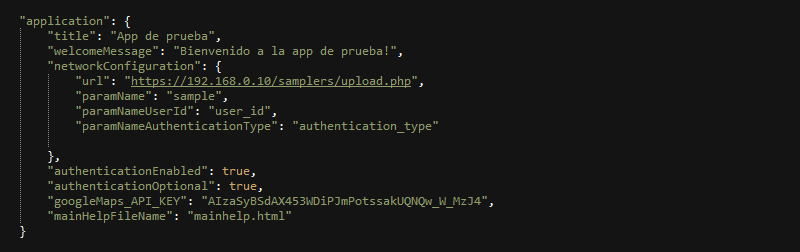
\includegraphics[scale=0.6]{50-anexos/B-uso/json_application.png} 
    \caption{Ejemplo del objeto application.}
\end{figure}	
	
	
\subsection{El objeto workflow}
	El objeto workflow representa el protocolo para la toma de la muestra. Son los pasos que se ejecutarán para tomar la misma.
	El objeto cuenta con dos campos:
		
	\begin{itemize}
	
		\item \textbf{actionLabel}: Un String con el título que se usará para el botón que inicia la activity TakeSampleActivity, que es la encargada de tomar la muestra.
		
		\item \textbf{steps}: Un Array de Objetos Step los cuales forman el workflow. El primer objeto del array se considera como el inicio del mismo. Ver la sección Steps para mas detalles.
	
	
	\end{itemize}	
	
	
\begin{figure}[H]
  \centering
    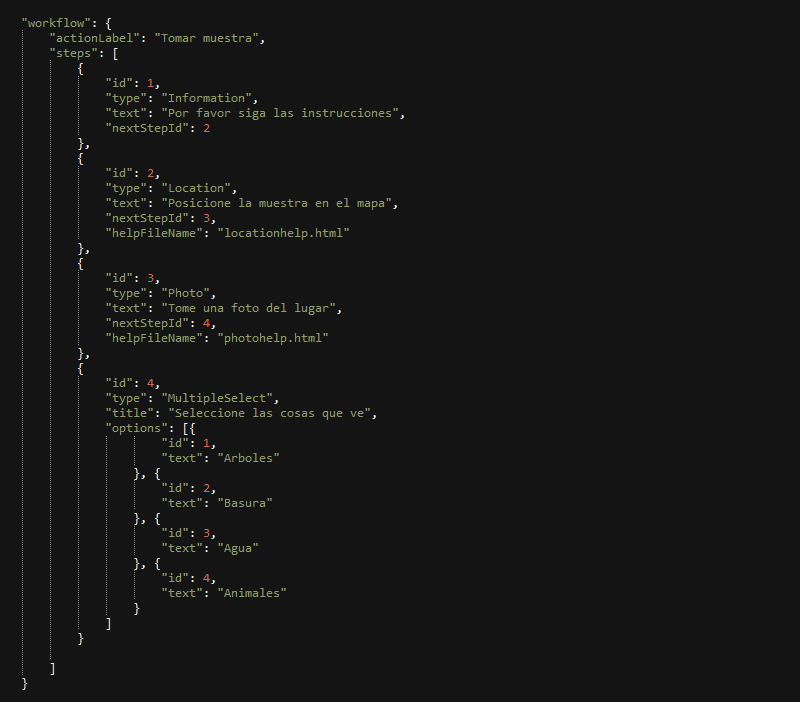
\includegraphics[scale=0.6]{50-anexos/B-uso/json_workflow.png} 
    \caption{Ejemplo del objeto workflow.}
\end{figure}	
		



\section{Mostrar Ayuda} \label{sec:mostrar_ayuda}
Samplers permite mostrar ayuda para el usuario final de la app a través de archivos HTML. Estos archivos deben estar ubicados junto con el archivo SamplersConfig.json

Samplers permite dos formas de mostrar ayuda:

\begin{itemize}

	\item \textbf{Ayuda general}: que se accede desde el menú de la Activity principal cuando se configura un archivo de ayuda para la app.
		
	\item \textbf{Ayuda puntual para cada Step}: que se accede desde un botón en los StepFragments que aparece cuando el Step tiene configurado un archivo de ayuda.

\end{itemize}


\begin{figure}[H]
  \centering
    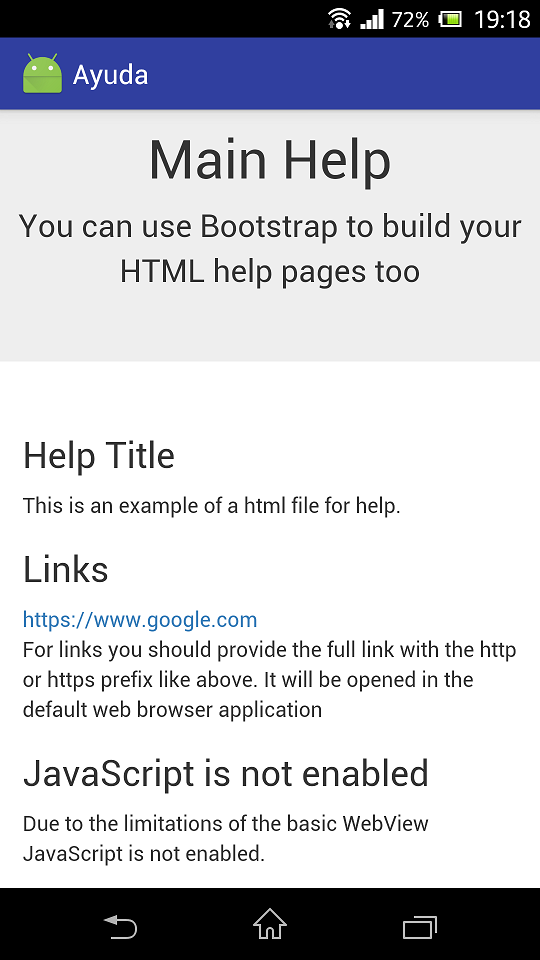
\includegraphics[scale=0.3]{50-anexos/B-uso/ayuda_ejemplo.png} 
    \caption{Ejemplo de como se muestra la ayuda.}
\end{figure}	
		

\textbf{JavaScript no esta habilitado:} Debido a las limitaciones del componente WebView de Android no esta habilitado el uso de JavaScript. Para más información ver la documentación oficial de Android sobre WebView.\footnote{https://developer.android.com/reference/android/webkit/WebView}

\subsection{Ayuda general}
Para configurar la ayuda general se debe completar el atributo \textit{mainHelpFileName} del objeto \textit{application} con el nombre del archivo HTML que contiene la ayuda que se quiere mostrar. El archivo HTML debe estar ubicado junto con el archivo SamplersConfig.json.

\begin{figure}[H]
  \centering
    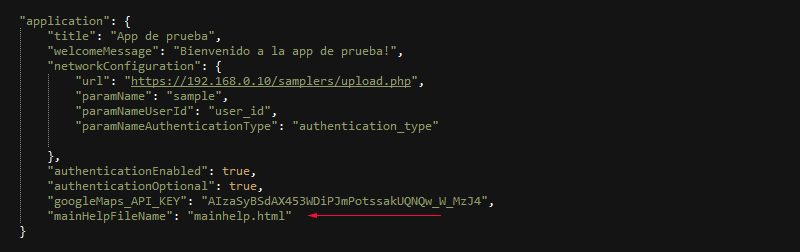
\includegraphics[scale=0.6]{50-anexos/B-uso/json_application_ayuda.png} 
    \caption{Ejemplo de configuración de ayuda general.}
\end{figure}	

\subsection{Ayuda puntual para cada Step}
Para configurar la ayuda para un Step se debe completar el atributo \textit{helpFileName} del objeto \textit{step} con el nombre del archivo HTML que contiene la ayuda que se quiere mostrar. El archivo HTML debe estar ubicado junto con el archivo SamplersConfig.json.

\begin{figure}[H]
  \centering
    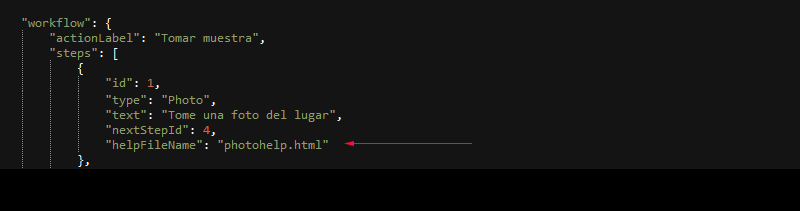
\includegraphics[scale=0.6]{50-anexos/B-uso/json_step_ayuda.png} 
    \caption{Ejemplo de configuración de ayuda en un Step.}
\end{figure}	


\section{Usando identificación} \label{sec:usando_autenticacion}
Por defecto Samplers provee identificación con Google, porque en Android es necesario tener una cuenta de Google para usar el dispositivo móvil, aunque también está preparado para poder integrar identificación con otras plataformas/APIs.

Para usar la identificación con Google, es necesario registrar la aplicación en la pagina de desarrolladores de google\footnote{https://developers.google.com/identity/sign-in/android/start-integrating}. Ahí hay que seguir los pasos para configurar la API en el proyecto dentro de la consola de Google. Es necesario proveer el nombre de la aplicación, package name, y también el SHA-1 hash del certificado con el que se firma la aplicación.

Una vez registrada la aplicación en Google, hay que configurar Samplers para habilitar la identificación como se explican en las secciones \ref{sec:identificacion_gradle} o \ref{sec:identificacion_manual}.

Una vez configurado los valores de los parámetros de identificación, Samplers mostrará un fragment de inicio de sesión la primera vez que el usuario intente tomar una muestra. Si la identificación es opcional, se mostrará un botón para omitir el inicio de sesión y continuar con la toma de la muestra. También se muestra un botón para iniciar sesión en la activity principal (si se está usando la que provee Samplers).

Cuando la muestra es enviada, el id de usuario y el método de identificación (por defecto 'google') se envían junto con esta.


\subsection{Configurar identificación con el generador de clases de Gradle} \label{sec:identificacion_gradle}

Para usar identificación usando el generador de clases de Gradle, es necesario configurar los siguientes parámetros en el objeto \textbf{applicaction}:

\begin{itemize}

	\item \textbf{authenticationEnabled}: poner en true para habilitar la identificación
		
	\item \textbf{authenticationOptional}: poner en true si se desea que la identificación sea opcional, o en false si se desea que la identificación sea obligatoria.
	
	\item Dentro del parámetro \textbf{networkConfiguration} es necesario establecer los parámetros \textbf{paramNameUserId} y \textbf{paramNameAuthenticationType} con los nombres de los parámetros con los que irán el id de usuario y el tipo de identificación usada respectivamente dentro del mensaje HTTP POST.
	

\end{itemize}

\begin{figure}[H]
  \centering
    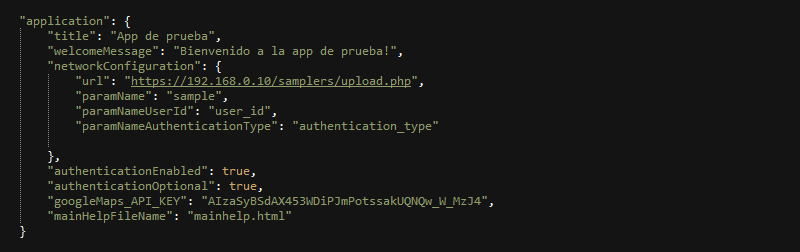
\includegraphics[scale=0.6]{50-anexos/B-uso/identificacion.png} 
    \caption{Ejemplo del objeto application configurado para usar identificación.}
\end{figure}	


\subsection{Configurar identificación manualmente} \label{sec:identificacion_manual}

Para usar identificación cuando se usan las clases directamente, es necesario definir la configuración de red y de identificación en el método \textbf{onCreate()} de la activity principal:

\begin{figure}[H]
  \centering
    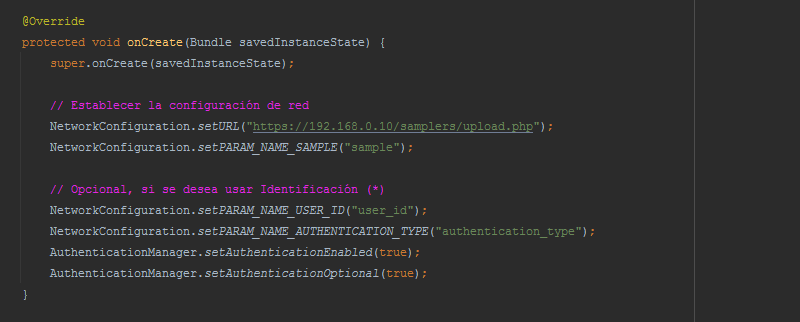
\includegraphics[scale=0.6]{50-anexos/B-uso/identificacion_manual.png} 
    \caption{Ejemplo de configuración de identificación en el método onCreate.}
\end{figure}	


\subsection{Usando un método de identificación propio} \label{sec:usar_auth_propia}

Con Samplers también se puede usar un método de identificación propio, definiendo un LoginFragment y una clase User (o varias clases si se desea proporcionar identificación con diferentes APIs, como Facebook, Instagram, Tweeter, etc.) y Samplers enviará junto con la muestra el id de usuario y el método de identificación usado.


\subsubsection{Definiendo un Login Fragment propio}

Es necesario crear un fragment que herede de LoginFragment, y configurar la clase AuthenticationManager para que lo use, llamando al método setLoginFragmentClass() dentro del método onCreate() de la ativity principal:

\begin{figure}[H]
  \centering
    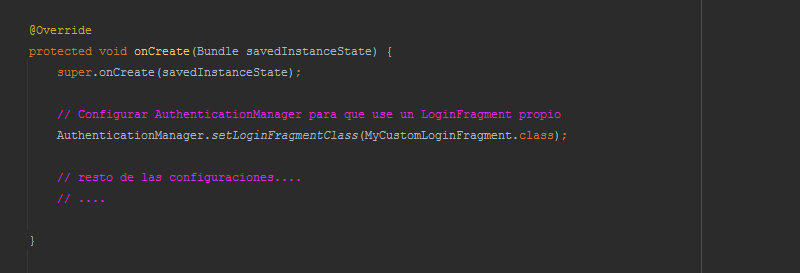
\includegraphics[scale=0.6]{50-anexos/B-uso/identificacion_propio_configurar.png} 
    \caption{Ejemplo de como configurar un LoginFragment propio.}
\end{figure}	


El proceso de login y la interacción con las APIs responsabilidad del desarrollador, pero después de que el usuario inicia sesión en la API seleccionada, es necesario llamar al método login() en la clase AuthenticationManager y al método onLogin() en el objeto mListener heredado:

\begin{figure}[H]
  \centering
    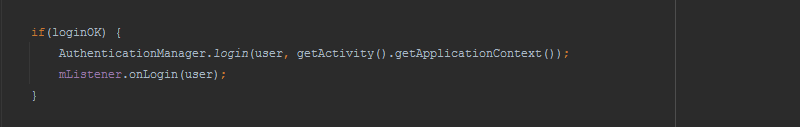
\includegraphics[scale=0.6]{50-anexos/B-uso/identificacion_loginOk.png} 
    \caption{Ejemplo de como llamar al método onLogin.}
\end{figure}	



\subsubsection{Definiendo una clase User propia}

Es necesario crear una clase usuario propia que implemente la interfaz User por cada método de identificación que se use. Los objetos de dichas clases se usarán para llamar al método login() de la clase AuthenticationManager.

\begin{figure}[H]
  \centering
    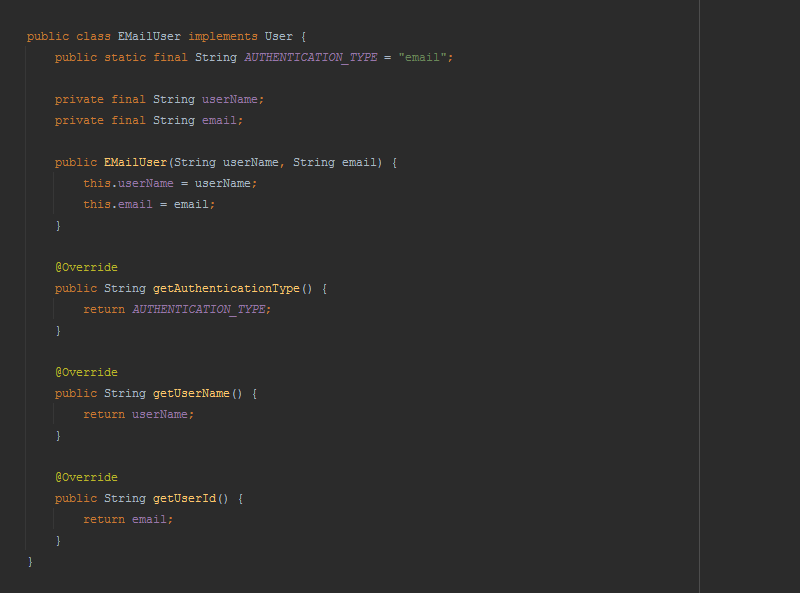
\includegraphics[scale=0.6]{50-anexos/B-uso/identificacion_user_propio.png} 
    \caption{Ejemplo de una clase usuario propia.}
\end{figure}	




\begin{comment}

\section{Personalización}

\subsection{Temas y colores}

\subsection{Idiomas}

\end{comment}

